\documentclass[11pt,a4paper]{article}

\usepackage[utf8]{inputenc}
\usepackage{amsmath,amssymb}
\usepackage{graphicx}
\usepackage{subcaption}
\usepackage{float}
\usepackage{hyperref}
\usepackage{geometry}
\usepackage{setspace}
\usepackage{booktabs}
\usepackage{tabularx}
\geometry{a4paper, margin=2.5cm}
\onehalfspacing

% We embed the GAP number directly into the title block, pushing it to the right 
% and adding a bit of vertical space before the actual title begins.
\title{
    \hfill {\normalsize \textbf{GAP-2026-041}} \\[2em]
    Azimuthal Asymmetries in Extensive Air Showers: UMD–SD Comparison and Insights into the Surface-Detector Sign Inversion
}
\author{Lautaro Silva Pizzi, Juan Manuel Figueira and Federico S\'anchez \\ Pierre Auger Observatory}
\date{August 2026}

\begin{document}
\maketitle

\begin{abstract}
We present a phenomenological study of the early--late azimuthal asymmetry of extensive air showers, extending this analysis for the first time to the Underground Muon Detector (UMD) of the Pierre Auger Observatory. Using a set of \texttt{CORSIKA}/\texttt{Offline} simulations of proton-induced showers with the \texttt{Sibyll,2.3e} hadronic interaction model in the energy range $\log_{10}(E/\mathrm{eV})\in[17.5,18.0]$, we compare the azimuthal modulation of the muonic component observed at the surface and underground. At large core distances, we find a pronounced difference between the two detectors: while the Surface Detector (SD) signal undergoes a sign inversion of the first-harmonic amplitude $A_1$, the UMD muon signal remains positive and follows a smooth evolution with radial distance and shower inclination. A decomposition of the SD signal shows that the electromagnetic component remains strongly positive, whereas the muonic component drives the sign inversion at large radial distances. The observed difference is consistent with the combined effect of the low-energy muon population and the distinct geometrical response of the two detectors. The $\sim540~\mathrm{g/cm^2}$ soil overburden of the UMD suppresses low-energy, highly divergent muons, while its approximately planar buried geometry avoids the side-wall exposure and track-length effects inherent to the volumetric water-Cherenkov tanks of the SD. The UMD therefore provides a phenomenologically cleaner probe of muon-induced azimuthal asymmetries and of the longitudinal development of extensive air showers. These results motivate the development of UMD-based asymmetry observables as complementary probes of the mass composition of ultra-high-energy cosmic rays.
\end{abstract}

\section{Introduction}
\label{sec:intro}

The azimuthal asymmetry of the particle density footprint at ground level has long been recognised as a sensitive probe of the longitudinal development of extensive air showers (EAS). Early phenomenological studies by Pryke \cite{Pryke1998} and by Billoir and collaborators \cite{Billoir2002, GAP2000_017}, later extended by Dembinski et al. \cite{GAP2007_124}, established the analytical framework in which the ground densities of inclined showers are parametrised by a first-order harmonic modulation and identified attenuation and geometric projection as its two leading sources. In this framework, the particle density $S$ in the shower plane is expressed as:

\begin{equation}
    S(r, \phi) = \langle S(r)\rangle \big[ 1 + A_1(r, \theta) \cos \phi \big] ,
    \label{eq:harmonic_fit}
\end{equation}
%
where $\langle S(r)\rangle$ is the azimuthally averaged density at radial distance $r$, and $A_1(r, \theta)$ is the amplitude of the early--late modulation. Following this convention, $A_1 > 0$ corresponds to a density peak in the early region, while $A_1 < 0$ corresponds to a density peak in the late region. The $\sin \phi$ term is omitted, as it averages to zero for isotropic arrival directions, and the expansion is truncated at first order because higher-order harmonics remain small in the targeted parameter space.

More recently, and in the context of the AugerPrime upgrade \cite{AugerPrime2016}, Bradfield \cite{BradfieldThesis} performed a comprehensive systematic study of asymmetries using both the Water Cherenkov Detector (WCD) and the Surface Scintillator Detectors (SSD), confirming the utility of azimuthal modulations as a mass-composition observable.

All of these analyses share a common limitation: the Surface Detector (SD) measures a signal combining the electromagnetic (EM) and muonic components of the cascade, and does so through a three-dimensional water volume with non-negligible side-wall exposure. As a consequence, SD-based asymmetry observables exhibit non-trivial features, including a suppression of the amplitude for deeply developing showers and an outright sign inversion of $A_1$ at large radial distances \cite{BradfieldThesis, Luce_ICRC2021, GAP2000_017}. Disentangling the mechanisms behind this inversion requires a detector that is intrinsically sensitive to the muonic component only and whose geometrical response is as close to planar as possible.

The purpose of this work is twofold. First, we extend the asymmetry analysis pioneered on the SD to the UMD, a study not previously reported. The UMD, part of the AMIGA extension~\cite{Botti2019, auger2020umd_infill}, consists of segmented plastic scintillators buried $2.3$~m underground. The resulting approximately $\sim 540~\mathrm{g/cm^2}$ soil overburden imposes an effective muon energy threshold of $E_\mu \gtrsim 1 ~\mathrm{GeV}/\cos\theta$, acting as an energy filter of incoming muons whose selectivity itself depends on zenith angle. Equally important, the buried scintillator plane presents a nearly two-dimensional detection geometry, which is qualitatively distinct from the cylindrical WCD tanks of the SD. Second, by exploiting a controlled Dense Ring topology together with the continuous radial spectrum of the SD-750 array, we contrast the phenomenology of the UMD signal against that of the SD, providing an empirical characterisation of the SD muon inversion reported in~\cite{Luce_ICRC2021, GAP2000_017}. A discussion of the possible physical mechanisms responsible for the qualitatively different behaviour of the two detectors is deferred to Section~\ref{sec:conclusions}.

We restrict our analysis to proton-initiated showers in the energy range $\log_{10}(E/\mathrm{eV}) \in [17.5, 18.0]$ simulated over the zenith range $\theta \in [0^\circ, 65^\circ]$. The note is structured as follows. In Section~\ref{sec:physics}, we review the well-established physical sources of azimuthal asymmetry. In Section~\ref{sec:methodology}, we detail the Monte Carlo (MC) production parameters and the evaluation topologies. Section~\ref{sec:results} presents the phenomenological results, contrasting the intrinsic asymmetry of the UMD with the convolved SD signal, and Section~\ref{sec:conclusions} summarises our findings, discusses plausible interpretations and outlines their implications for future mass-composition studies.

\section{Physical Sources of Azimuthal Asymmetries}
\label{sec:physics}

Before quantifying the asymmetry, it is convenient to distinguish the two reference frames involved in the analysis: the ground plane (topographic frame) and the shower plane, defined as the plane orthogonal to the shower axis. The radial distance to the core $r$ and the azimuthal angle $\phi$ are defined strictly in the shower plane throughout this work, as illustrated in Figure~\ref{fig:shower_plane}.

For a vertical shower ($\theta = 0^{\circ}$), the two frames coincide and the particle density is, up to shower-to-shower fluctuations and small deflections induced by the geomagnetic field, symmetric around the shower axis. Consequently, iso-density contours at ground level are circles centred on the core. The core is defined as the position where the axis along which the shower evolves intersects with the ground. Vertical showers are therefore taken as the reference configuration with no azimuthal asymmetry.

\begin{figure}[h]
\centering
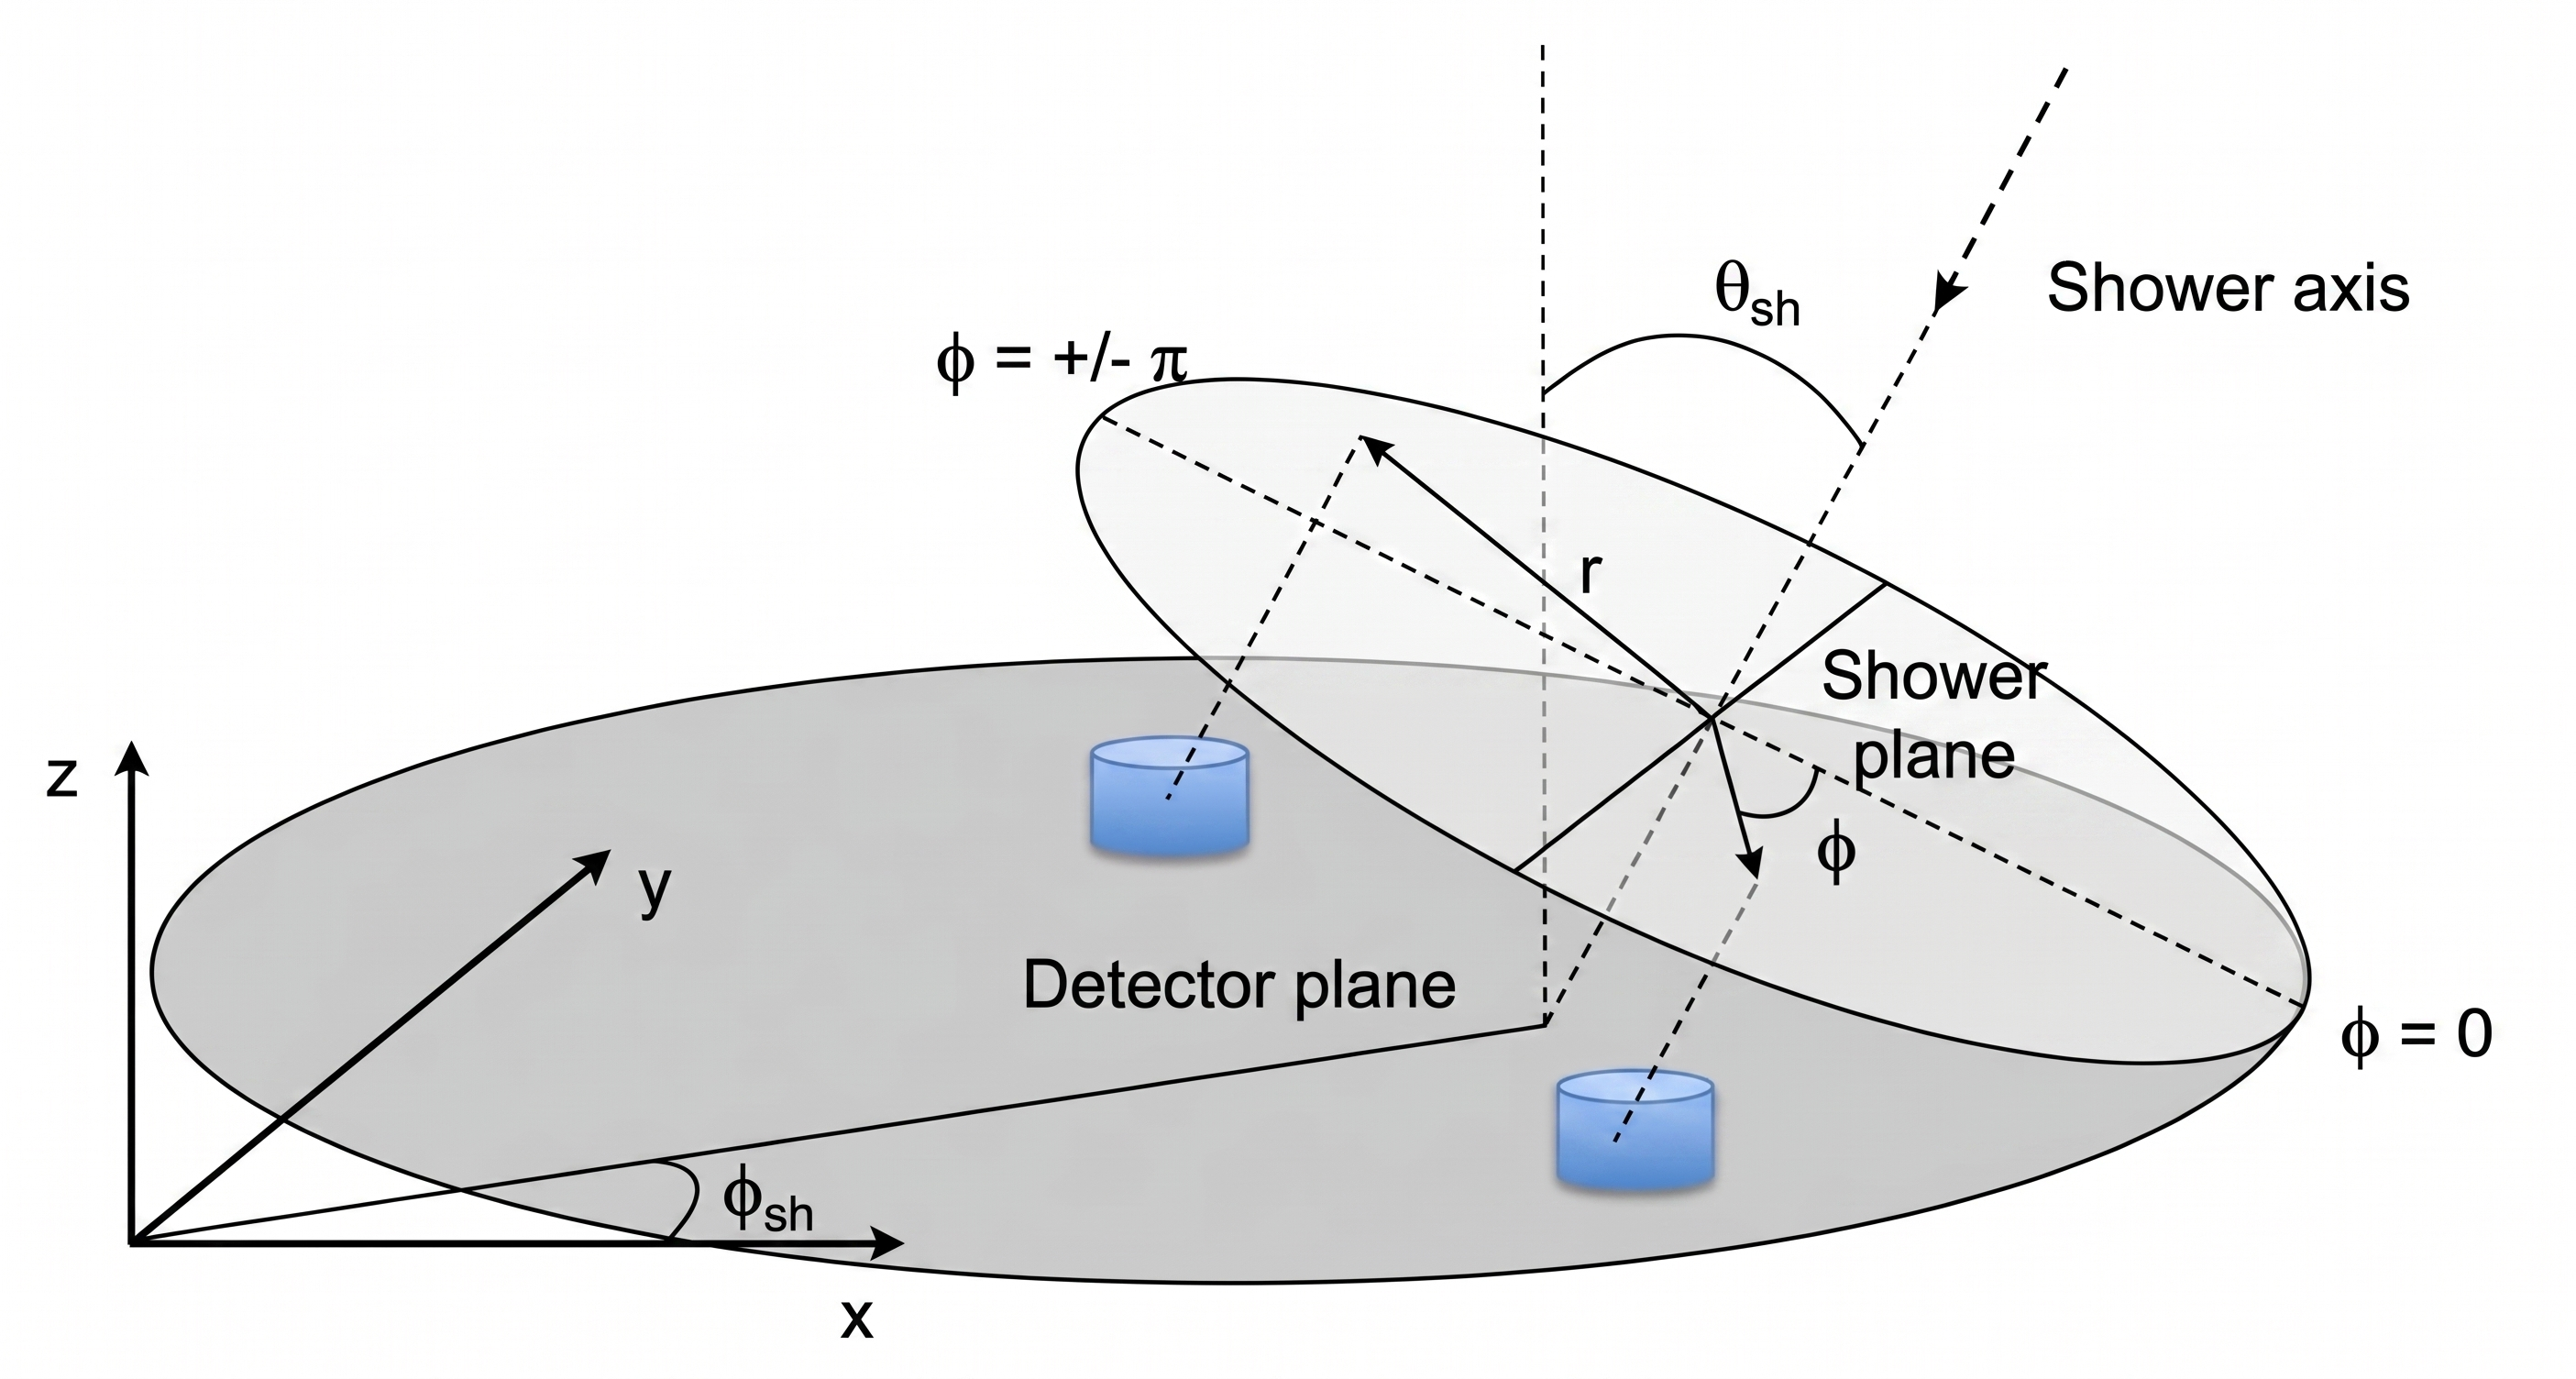
\includegraphics[width=1\textwidth]{esquema_lluvia.jpeg}
\caption{Geometric schematic of an EAS. Detector positions on the ground plane are projected onto the shower plane to define the intrinsic coordinates $r$ and $\phi$.}
\label{fig:shower_plane}
\end{figure}

For an inclined primary ($\theta > 0^{\circ}$), the shower plane is tilted with respect to the ground, breaking the circular symmetry from the point of view of an observer on the array (see Figure~\ref{fig:shower_plane}). Two azimuthal regions are conventionally defined for detectors located at the same radial distance $r$ in the shower plane:

\begin{itemize}
\item \textbf{Early region ($\phi \approx 0^{\circ}$):} the section of the shower front closest to the ground, where particles impact the array first and traverse the shortest atmospheric slant depth.
\item \textbf{Late region ($\phi \approx \pm 180^{\circ}$):} the diametrically opposite section, i.e., the section of the shower front which remains elevated when the early side has already hit the ground. Particles here propagate through a larger atmospheric depth before detection.
\end{itemize}

The resulting azimuthal modulation reflects the superposition of two well-established competing physical mechanisms, which we now review.

\subsection{Mechanisms Driving the Early Excess}
\label{subsec:early_excess}

Two independent physical phenomena act to increase the particle density in the early region relative to the late region, driving a positive asymmetry.

\subsubsection{Atmospheric Attenuation}

Because the late region of an inclined shower is more elevated relative to the ground than the early region, particles travelling towards $\phi \approx \pm 180^{\circ}$ traverse a larger atmospheric depth than those arriving at $\phi \approx 0^{\circ}$. As the cascade develops and its particle content is progressively absorbed, this asymmetric slant depth translates into a density excess in the early direction and a deficit in the late direction~\cite{Pryke1998,dova2003,BradfieldThesis}. While muons are considerably more penetrating than the EM component, at the energies relevant for the UMD, both energy losses and muon decay in flight produce a sizeable positive contribution to the early-late asymmetry.

\subsubsection{Geometrical Flux Projection}

As originally noted by Billoir \cite{GAP2000_017}, an event that is perfectly symmetric in the shower reference frame will appear asymmetric when projected onto the ground plane. Particles hitting the ground in the early region intersect the ground plane more perpendicularly than those in the late region, thereby presenting a larger cross-sectional flux per unit area. Bertou and Billoir parametrised the angular modulation of this specific projection as

\begin{equation}
    \mathcal{A}_{geo}(r, \phi, \theta) = A_{geo}(r, \theta) \cos \phi
    \label{eq:geometric_effect_full}
\end{equation}
%
where the radial-dependent amplitude is defined as \cite{GAP2000_017}:

\begin{equation}
    A_{geo}(r, \theta) = \left\langle \frac{p_t(r)}{-p_z(r)} \right\rangle \tan \theta
    \label{eq:geometric_effect}
\end{equation}
%
where $p_t$ and $p_z$ are the transverse and longitudinal momentum components, respectively. We adopt the convention that $p_z < 0$ for downward-going particles. Therefore, the denominator $-p_z$ is positive. Since $p_t$ and $\tan\theta$ are also positive, the amplitude $A_{geo}$ is strictly positive, yielding a local maximum in the early region ($\phi = 0^\circ$). Thus, the geometric flux projection acts additively with atmospheric attenuation to drive a positive asymmetry.

\subsection{Beyond Attenuation and Geometry}
\label{subsec:beyond}

The two mechanisms discussed above, atmospheric attenuation and geometric projection onto a flat ground plane, both drive a strictly positive first-harmonic amplitude. They therefore cannot, on their own, account for the sign inversion of $A_1$ that has been reported for the SD signal at large radial distances \cite{BradfieldThesis, Luce_ICRC2021, GAP2000_017}. The existence of this inversion suggests that at least one additional effect, either intrinsic to the shower physics or associated with the specific response of the detector, must be operative, and one whose contribution grows in importance at large core distances and inclined geometries. The phenomenological characterisation of this competition is the central subject of the present work; a discussion of the mechanisms that plausibly account for the observed behaviour is deferred to Section~\ref{sec:conclusions}, once the empirical evidence has been presented.

\subsection{Geomagnetic Deflection}
\label{subsec:geomagnetic}

The Earth's magnetic field ($\vec{B}$) exerts a Lorentz force on the charged components of the cascade~\cite{Scornavacche2026,collaboration_2014}, laterally separating $\mu^{+}$ and $\mu^{-}$. Because the Observatory receives an essentially isotropic flux, the relative orientation of $\vec{B}$ with respect to the shower plane varies from event to event. In a global harmonic fit, this variability introduces an incoherent variance that dilutes the early--late modulation. For the intermediate zenith-angle range ($\theta \lesssim 65^{\circ}$) and the energy interval considered here, the geomagnetic contribution is expected to be a second-order effect and is neglected in the following analysis.

\section{Simulation Datasets and Array Topologies}
\label{sec:methodology}

\subsection{Simulation Framework}
\label{subsec:framework}

The data analysed in this work originate from the official Pierre Auger Collaboration production \textit{Offline\,icrc2025-test7: SD-750 and UMD production for Auger}. Air showers were generated with \texttt{CORSIKA} (v7.8010) \cite{heck1998} and processed through the \texttt{Offline} framework, which simulates the detector responses of the WCD-based SD-750 array and of the associated UMD modules. The primary simulation parameters are summarised in Table~\ref{tab:mc_params}.

\begin{table}[h]
\centering
\caption{Summary of Monte Carlo simulation and array parameters.}
\label{tab:mc_params}
\begin{tabularx}{0.8\textwidth}{X c}
\toprule
\textbf{Parameter} & \textbf{Value} \\
\midrule
CORSIKA Version & 7.8010 \\
High-Energy Hadronic Model & Sibyll 2.3e \cite{riehn2020} \\
Low-Energy Hadronic Model & FLUKA \\
Energy Range & $\log_{10}(E/\text{eV}) \in [17.5, 18.0]$ \\
Zenith Range & $\theta \in [0^\circ, 65^\circ]$ (10 equal $\sin^2\theta$ bins) \\
Thinning Level & $10^{-6}$ \\
Geomagnetic Field & Malarg\"ue  \\
Primary Species & Proton \\
Showers per Primary & $\approx 24,000$ \\
\bottomrule
\end{tabularx}
\end{table}

To ensure statistical robustness and homogeneity in the harmonic fits, the present analysis is restricted to the complete \texttt{Sibyll\,2.3e} subset, which is the set of simulations that provides the most statistics with $\sim24,000$ proton-initiated showers. 

To disentangle the intrinsic physical asymmetry from the systematic angular smearing introduced by the standard reconstruction pipeline, we bypass the reconstructed variables. Instead, we compute the station coordinates in the shower plane analytically from the Monte Carlo truth, taking the injected MC core as the origin, we apply a 3D Euler rotation defined by the true MC zenith and azimuth to project the surface stations onto the true shower plane. This manual geometrical projection was applied to the 750~m Array stations, while Dense Ring stations natively operate in a relative frame and do not require these manual geometry rotations. The results presented here thus represent the intrinsic physical asymmetry of the cascade.

\subsection{Evaluation Topologies: Dense Ring and 750~m Array}
\label{subsec:topologies}

To systematically deconstruct the mechanisms governing the ground-level signal, the analysis is performed across two complementary spatial configurations.

\subsubsection{The Dense Ring}
To study the azimuthal modulation while decoupling it from the radial fall-off of the LDF, a strictly controlled geometry is required. In the simulation, the shower core is surrounded by a ring of 12 stations placed at a fixed radial distance $r = 450$~m, azimuthally equispaced by $30^{\circ}$ in the shower plane. To increase the effective statistics, a resampling technique is applied whereby the \texttt{Offline} framework executes five reconstruction iterations per \texttt{CORSIKA} shower, each with a displaced core. By construction, any observed azimuthal modulation in this ring is attributable solely to physical effects that depend on $\phi$, allowing a clean extraction of $A_1$.

\subsubsection{The SD-750 Array}
While the Dense Ring isolates the azimuthal behaviour at a single reference radius, it does not probe the continuous spatial evolution of the cascade. To map the transition from the near-core to the far-core regime, the analysis is scaled to the realistic topology of the 750~m array. By combining the true MC geometry projection with the array topology, we observe how the azimuthal modulation of $A_1$ evolves as a function of the distance to the shower axis.

\section{Phenomenological Results: UMD vs.\ SD}
\label{sec:results}

Throughout this section, the amplitude $A_1$ is extracted from unweighted least-squares fits of Eq.~\eqref{eq:harmonic_fit} using the true MC geometry projection.

\subsection{Pure Muon Phenomenology in a Controlled Environment}
\label{subsec:dense_ring_results}

The analysis begins within the controlled geometry of the Dense Ring, evaluating stations at a fixed radial distance of $r = 450$~m. This configuration isolates the azimuthal modulation from the radial fall-off of the lateral distribution function.

Before examining the global evolution of the asymmetry, it is instructive to visualise how the modulation manifests at the individual detector level. By dividing the signal $S(r, \phi)$ of each virtual station by the azimuthally averaged density $\langle S(r) \rangle$ of the ring, we can factor out the absolute particle density and isolate the pure harmonic modulation $[1 + A_1 \cos \phi]$.

Figure~\ref{fig:example_fit} displays this normalised signal $S/\langle S \rangle$ as a function of the shower-plane azimuthal angle $\phi$ for the MC UMD muons ($N_\mu^{\mathrm{MC}}$) in a highly inclined zenith bin. The data exhibits a clear and robust harmonic behaviour, peaking unambiguously in the early region ($\phi = 0^\circ$) and reaching a minimum in the late region ($\phi = \pm 180^\circ$). The excellent agreement between the simulated data points and the first-order harmonic fit validates the parametrisation established in Eq.~\eqref{eq:harmonic_fit} and confirms that higher-order contributions are negligible in this regime, allowing for a rigorous extraction of the amplitude $A_1$.

\begin{figure}[h]
    \centering
    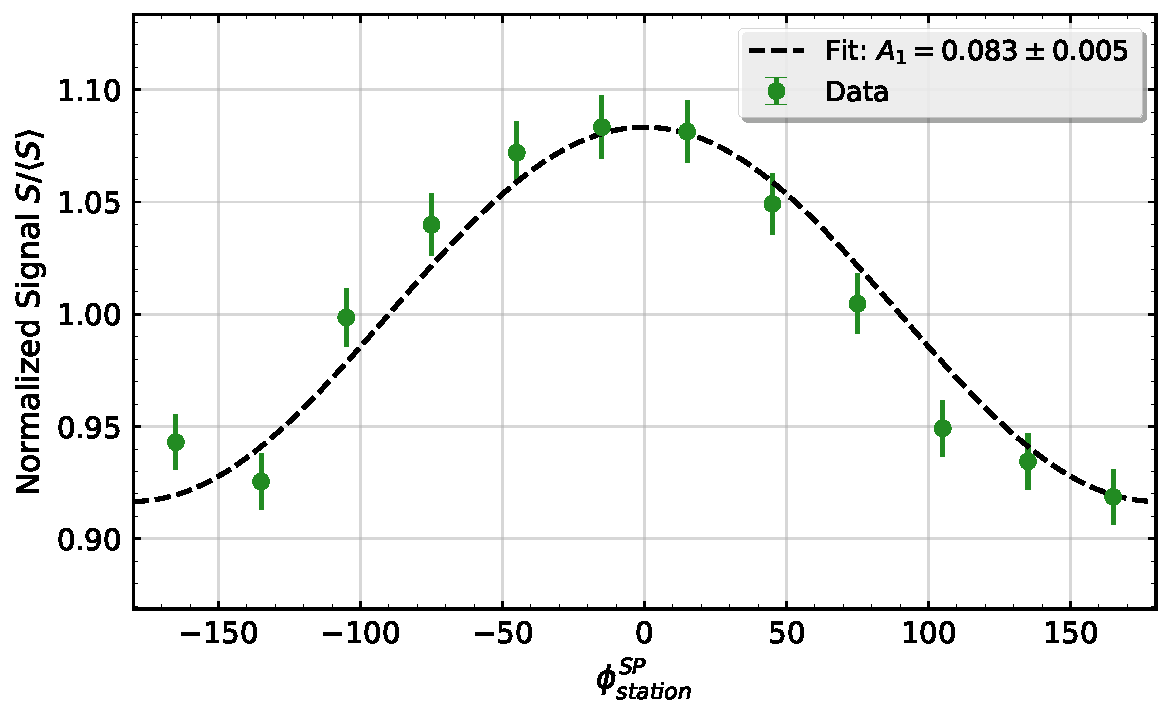
\includegraphics[width=1\textwidth]{Ajuste_UMD_MC_Bin9.pdf}
    \caption{Example of the first-order harmonic fit applied to the normalised MC muon density ($N_\mu^{\mathrm{MC}}$) in the Dense Ring topology ($r = 450$~m). The data corresponds to a representative highly inclined zenith bin. The signal exhibits a clear early excess ($\phi = 0^\circ$) and late deficit ($\phi = \pm 180^\circ$), yielding an asymmetry amplitude of $A_1 = 0.083 \pm 0.005$.}
    \label{fig:example_fit}
\end{figure}

Having established the robustness of the harmonic extraction, we now evaluate the evolution of the asymmetry amplitude $A_1$ as a function of the zenith angle $\theta$. Figure~\ref{fig:evolucion_asym_vs_theta} shows the evolution of $A_1$ as a function of the zenith angle $\theta$ for three observables: the reconstructed UMD muon counts ($N_\mu^{\mathrm{REC}}$), the true injected UMD muons ($N_\mu^{\mathrm{MC}}$) and the total SD signal in VEM units.

Two distinct regimes can be identified. For low and moderate inclinations ($\theta \lesssim 45^{\circ}$), not only does the SD amplitude significantly exceed that of the UMD, but it also grows faster. At moderate zenith angles the SD is dominated by the EM component, whose density is governed by bremsstrahlung and pair production and is therefore attenuated exponentially over a short radiation length. The steep longitudinal gradient of the EM cascade translates into a large positive asymmetry when projected onto the shower plane.

For high inclinations ($\theta \gtrsim 50^{\circ}$), the atmospheric slant depth grows rapidly ($\propto \sec\theta$). The EM component is largely absorbed before reaching the ground, and the SD signal becomes progressively muon-dominated. In this regime the SD amplitude drops sharply, reflecting both the reduced EM contribution and an additional suppression of the muonic asymmetry itself, whose physical origin will be discussed in Section~\ref{sec:conclusions}.

The UMD, which is by construction insensitive to the EM component, exhibits a smooth, monotonically increasing positive asymmetry that for higher inclinations shows a slight magnitude decrease, less pronounced than the drop observed in the SD. The UMD closely tracks the atmospheric attenuation of the high-energy muonic component of the shower, without being affected by either the electromagnetic depletion or by the additional mechanism that appears to suppress the SD amplitude at large zenith angles.

\begin{figure}[h]
\centering
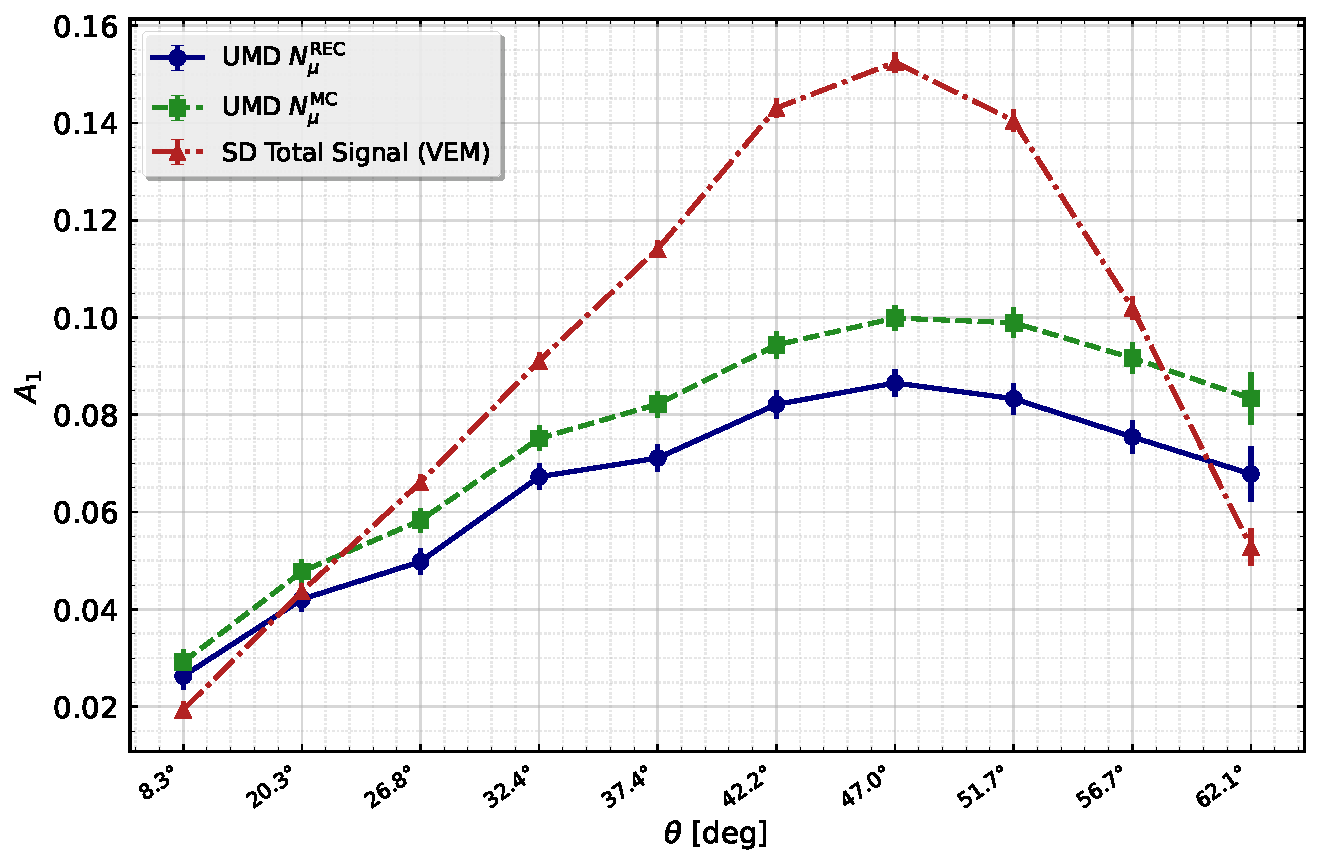
\includegraphics[width=1.0\textwidth]{Evolucion_Asimetria_vs_Theta.pdf}
\caption{Evolution of the first-harmonic amplitude $A_1$ as a function of the zenith angle $\theta$ in the Dense Ring topology ($r = 450$~m). The UMD is shown for reconstructed ($N_\mu^{\mathrm{REC}}$) and Monte Carlo true muons ($N_\mu^{\mathrm{MC}}$). The total SD signal in VEM units is also shown. A clear inversion of the hierarchy between the SD and the UMD is observed at high inclinations.}
\label{fig:evolucion_asym_vs_theta}
\end{figure}

\subsection{Radial Dynamics and the SD Sign Inversion}
\label{subsec:infill_results}

We now turn to the continuous radial spectrum provided by the 750~m array topology. Figure~\ref{fig:global_a1_umd_radial_zenith} shows the evolution of the UMD amplitude $A_1$, using the MC muons and coordinate system, as a function of the distance to the shower axis and the zenith angle. The amplitude increases both with radial distance, as expected from the growing difference in atmospheric slant depth between the early and late sides of the shower, and with inclination. For quasi-vertical showers ($\theta < 20^{\circ}$) the amplitude of the asymmetry is very close to zero.

The comparison of the UMD and the total SD signal in the 750~m array (Fig.~\ref{fig:umd_vs_sd_infill}) exposes a striking behavioural difference for the reference zenith bin $30^{\circ} \le \theta < 40^{\circ}$. The UMD amplitude grows smoothly towards positive values and plateaus at large $r$, in qualitative agreement with the expectation from atmospheric attenuation. In contrast, the total SD signal reaches a local maximum around $r \sim 700$~m and then drops sharply, crossing zero near $r \sim 1050$~m and becoming strongly negative at $r \gtrsim 1200$~m. This inversion is a genuine feature of the SD ground signal and its physical origin is the central puzzle addressed in this note.

\begin{figure}[h!]
    \centering
    \begin{subfigure}{1\textwidth}
        \centering
        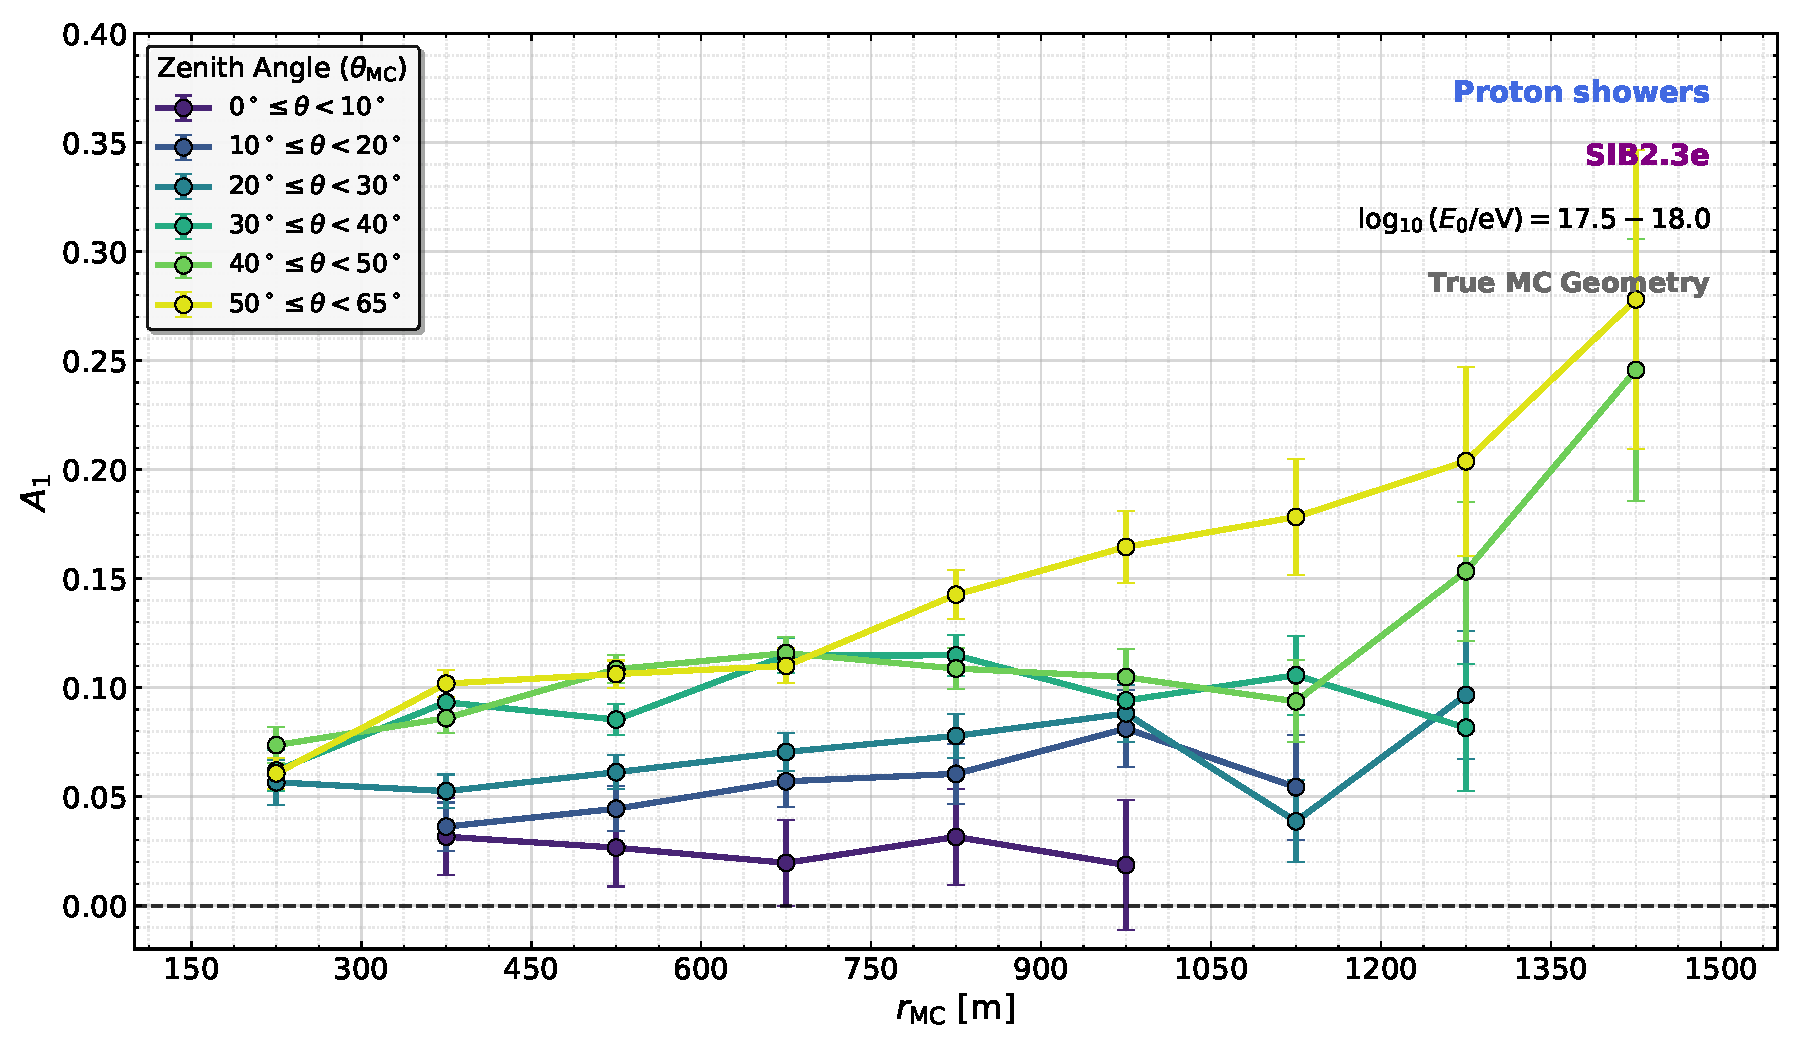
\includegraphics[width=0.94\textwidth]{Global_A1_vs_R_Theta_MC.pdf}
        \caption{}
        \label{fig:global_a1_umd_radial_zenith}
    \end{subfigure}
    \begin{subfigure}{1\textwidth}
        \centering
        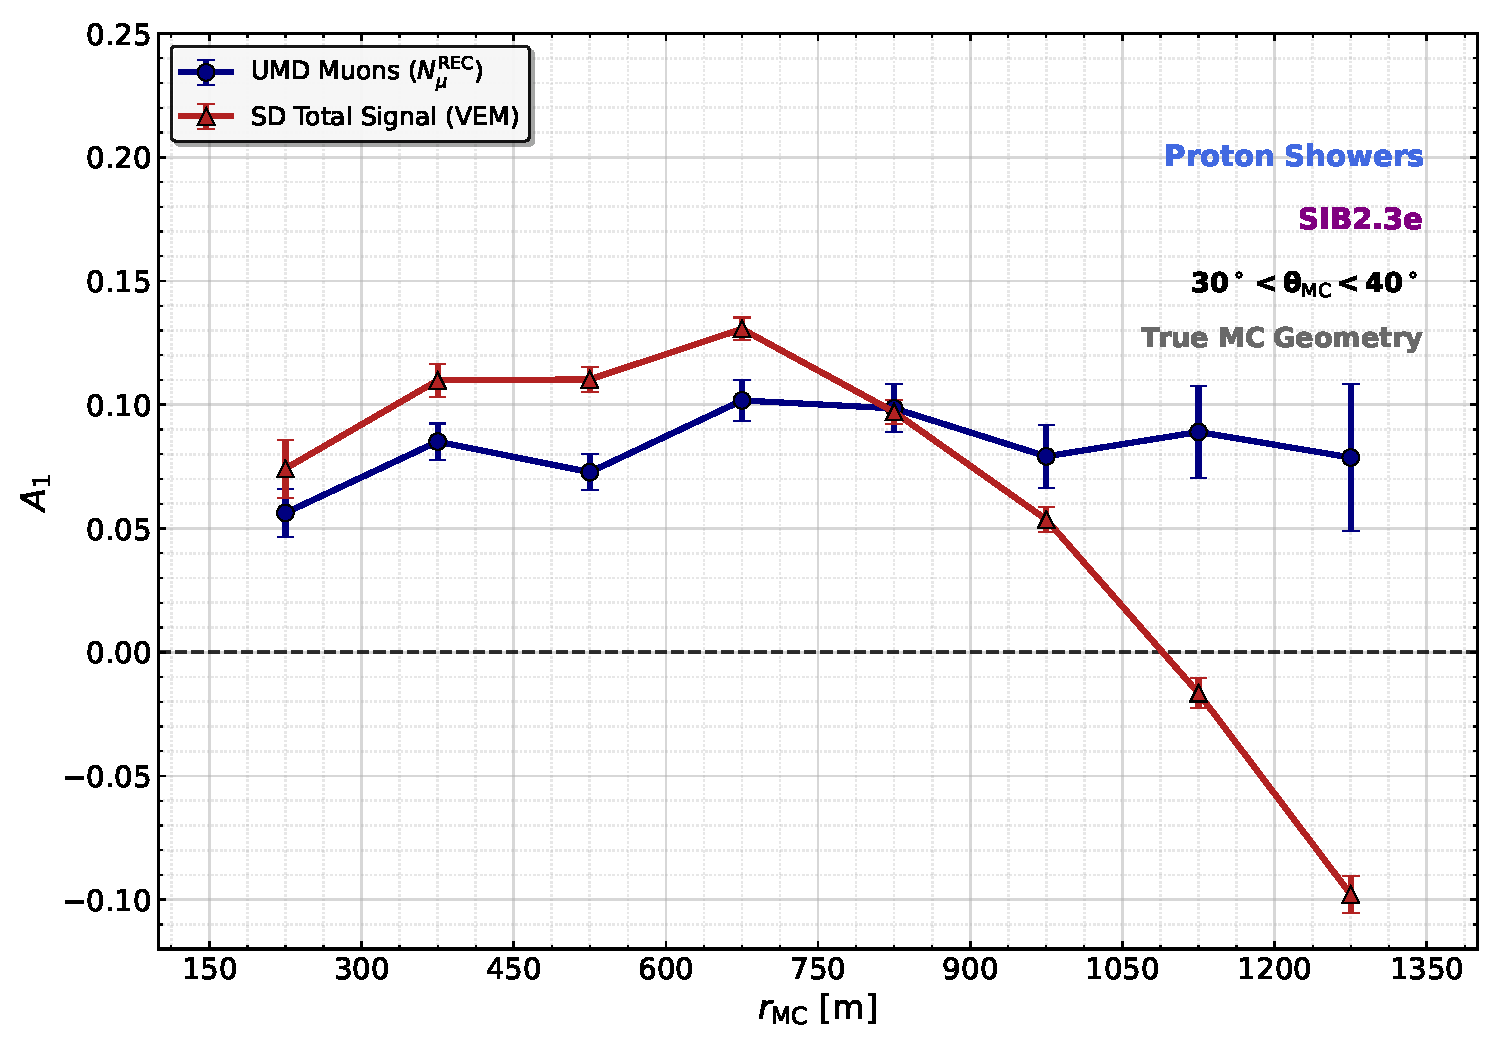
\includegraphics[width=0.94\textwidth]{UMD_vs_SD_Total_Asymmetry.pdf}
        \caption{}
        \label{fig:umd_vs_sd_infill}
    \end{subfigure}
    \caption{Top: Evolution of the UMD first-harmonic amplitude $A_1$ as a function of the distance to the shower axis across all evaluated zenith-angle bins. The amplitude grows monotonically with both radial distance and shower inclination. Bottom: Radial evolution of the first-harmonic amplitude $A_1$ comparing the pure muonic UMD signal ($N_\mu^{\mathrm{REC}}$) with the total SD signal (VEM) in the reference bin $30^{\circ} \le \theta < 40^{\circ}$. The UMD amplitude follows the attenuation-driven expectation, while the SD total signal undergoes a pronounced sign inversion in the far-core regime.}
\end{figure}
\vspace{4cm}

\subsection{Signal Dissection: EM vs.\ Muonic Contributions}
\label{subsec:signal_dissection}

To localise the physical origin of the SD inversion within the composite ground signal, we deconstruct the total VEM signal into its formative components at MC level: the EM and muon particle counts reaching the detector. Figure~\ref{fig:sd_dissection} shows the radial evolution of $A_1$ for each of these components in the same zenith bin $30^{\circ} \le \theta < 40^{\circ}$.

\begin{figure}[h]
\centering
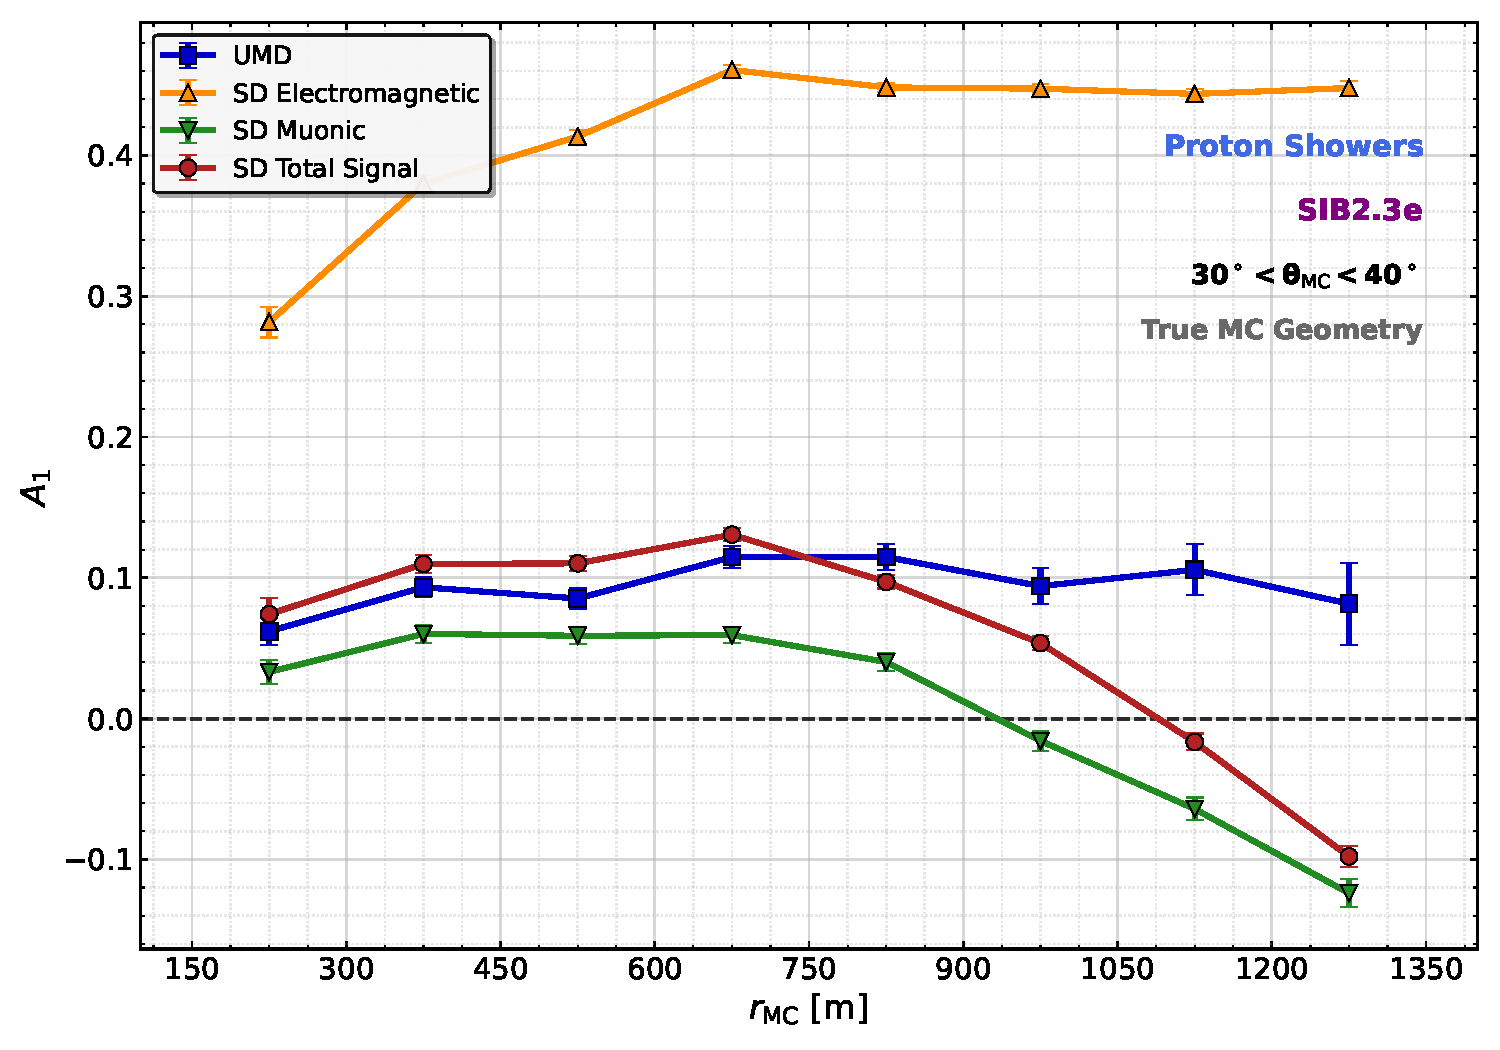
\includegraphics[width=1.0\textwidth]{SD_Desglose_Componentes_vs_UMD.pdf}
\caption{Deconstruction of the azimuthal asymmetry of the ground-level components compared with the UMD response in the reference bin $30^{\circ} \le \theta < 40^{\circ}$. The SD EM component shows a strongly positive attenuation asymmetry. The surface muons of the SD drive a negative inversion at large radial distances, while the UMD muons remain positive and stable.}
\label{fig:sd_dissection}
\end{figure}

The EM component displays a strongly positive asymmetry ($A_1 \sim 0.3$--$0.45$) across the whole radial range. Because EM particles are continuously produced and absorbed on short scales, their ground density is tightly coupled to the local longitudinal development of the cascade and is therefore a pure tracer of atmospheric attenuation.

The incident muons at the SD WCD, by contrast, drive the inversion. Near the core they behave similarly to the UMD muons and to the EM asymmetry, but for $r \gtrsim 750$~m the amplitude decreases rapidly and eventually crosses into the negative regime. Crucially, it must be noted that in the \texttt{Offline} simulation, $N_{\mu, \mathrm{sup}}^{\mathrm{MC}}$ represents the particle count incident on the three-dimensional volumetric boundaries of the WCD tank, rather than an ideal 2D ground plane. Consequently, its sign inversion already encapsulates detector-specific geometric biases, such as the differential exposure of the tank's side walls. Because the EM component is heavily depleted at large radii and inclined geometries, its relative contribution to the total signal becomes progressively negligible. As the total signal becomes dominated by the muonic component, the global SD asymmetry inherits this volumetric and kinematic sign inversion beyond $r \sim 1$~km, which is further exacerbated when converting particle counts to deposited energy (VEM).

The direct comparison with the UMD is particularly illuminating. Both detectors respond to the muonic component of the shower, yet they exhibit qualitatively opposite behaviour in the far-core regime: while the SD surface muons drive $A_1$ to negative values at large $r$, the UMD muons preserve a positive, essentially flat asymmetry across the whole accessible radial range. Two structural differences between the instruments stand out. First, their effective energy threshold for muons is very different: while the SD is sensitive to muons down to $\sim 100$~MeV kinetic energy at the WCD, the $\sim 540~\mathrm{g/cm^{2}}$ soil overburden of the UMD removes muons with $E_\mu \lesssim 1 ~\mathrm{GeV}/\cos\theta$ at ground level. Second, their detection geometry differs qualitatively: the SD WCD is a cylindrical water volume with a top surface and non-negligible side walls, while the UMD is essentially a buried scintillator plane with no vertical exposure. Both differences point to plausible mechanisms behind the observed contrast, which we develop further in the discussion of Section~\ref{sec:conclusions}.

Table~\ref{tab:a1_summary} summarises the observed amplitudes at three representative radii.

\begin{table}[h]
\centering
\caption{Summary of azimuthal asymmetry amplitudes ($A_1$) for $\theta \in [30^\circ, 40^\circ]$ at selected shower-plane radii. Statistical fit uncertainties are typically $\le 0.02$.}
\label{tab:a1_summary}
\begin{tabular}{l c c c}
\toprule
\textbf{Observable} & \textbf{$r = 450$~m} & \textbf{$r = 800$~m} & \textbf{$r = 1200$~m} \\
\midrule
SD-EM (MC) & $+0.40$ & $+0.45$ & $+0.44$ \\
SD-Muon (MC) & $+0.05$ & $+0.04$ & $-0.10$ \\
SD Total (VEM) & $+0.11$ & $+0.09$ & $-0.08$ \\
UMD $N_\mu^{\mathrm{MC}}$ & $+0.10$ & $+0.12$ & $+0.11$ \\
\bottomrule
\end{tabular}
\end{table}

\section{Conclusions and Discussion}
\label{sec:conclusions}

We have revisited the phenomenology of the early--late azimuthal asymmetry in extensive air showers and, for the first time, extended the analysis to the Underground Muon Detector of the AMIGA enhancement. The main empirical result of this work is a striking contrast between the two detectors: the UMD exhibits a smooth, positive and monotonic first-harmonic amplitude $A_1$ that grows with radial distance and shower inclination, reaching $A_1 \sim 0.11$ at $r = 1200$~m in the reference bin $30^\circ \le \theta < 40^\circ$; the total SD signal, in contrast, undergoes a pronounced sign inversion in the far-core regime, reaching $A_1 \sim -0.08$ at the same radius. Component-level deconstruction reveals that the EM contribution remains strongly positive ($A_1 \sim 0.4$) at all radii, while the SD surface muons alone drive the negative inversion at large $r$. Since atmospheric attenuation contributes a strictly positive amplitude, this inversion necessarily calls for additional mechanisms operative in the SD but absent in the UMD.

The empirical evidence suggests that the observed SD inversion is the result of two compounding mechanisms: a primary physical driver operating at the particle kinematics level, and a severe instrumental bias associated with the detector's volumetric geometry.

The first mechanism is kinematic and targets the low-energy portion of the muonic flux. Muons inherit from the parent hadronic interaction a bounded transverse momentum on the QCD scale, so that low-energy muons ($|p_z| \sim p_t$) are emitted with wide divergence angles while high-energy ones ($|p_z| \gg p_t$) remain collimated along the shower axis. Because the muon energy spectrum falls steeply as $E^{-2.6}$ \cite{Cazon2012}, the low-energy population is numerically dominant. The projection of its broad emission cone from an elevated production point onto an inclined ground plane plausibly generates a massive statistical particle-density excess in the geometrically farther, late region. The $\sim 540~\mathrm{g/cm^2}$ soil overburden of the UMD, which requires $E_\mu \gtrsim 1~\mathrm{GeV}/\cos\theta$ for detection, filters out precisely this divergent population, preserving only the collimated high-energy muonic backbone that faithfully tracks atmospheric attenuation. 

The second mechanism, following the analytical framework of Bertou and Billoir~\cite{GAP2000_017}, is strictly instrumental and acts as a compounding factor driven by the volumetric nature of the Water Cherenkov Detectors. The SD tanks present not only a top surface but also cylindrical side walls of appreciable height. The geometric asymmetry of the flux entering the tank through the sides includes a cross-term proportional to $(p_z/p_r) \cos\Phi \sin 2\theta$~\cite{GAP2000_017}, which contributes negatively to the overall harmonic asymmetry, actively reducing the early excess and favouring the late region. For highly inclined incoming particles, this lateral flux can even surpass the top-cover flux. Crucially, this geometric particle-count inversion is further exacerbated when converting to deposited energy (VEM) due to track-length effects. Muons entering through the lateral walls traverse, on average, longer paths through the water, depositing significantly more energy. Furthermore, even for muons entering through the top cover, those arriving from the late region have a larger local inclination angle ($\theta_{\text{local}}$) relative to the detector than those from the early region. Since the track length through the water scales as $1/\cos\theta_{\text{local}}$, these late-region muons deposit systematically more energy per particle, creating an additional artificial enhancement of the late-region VEM signal.

In summary, the UMD acts as a double filter , energetically removing the divergent low-energy muons, and geometrically eliminating the volumetric side-wall and track-length exposure of the SD, isolating the pure attenuation-driven asymmetry of the high-energy muonic cascade. Regardless of the relative quantitative weight of the kinematic and instrumental effects within the SD, our findings establish the UMD as a phenomenologically cleaner instrument for the study of azimuthal asymmetries. The ability to decouple the muonic attenuation asymmetry from both EM contamination and the complex mechanisms driving the SD inversion opens the door to its exploitation as an independent probe of the longitudinal development of the cascade and, ultimately, of the primary mass composition. New observables based on the muonic asymmetry could be developed by comparing results from proton- and heavy-nucleus-induced showers. These observables could be explored as tools to improve discrimination between light and heavy primaries. Furthermore, their correlations with established composition-sensitive observables, such as the surface muon density ($\rho_\mu$) and the depth of shower maximum ($X_{\max}$), could be studied to achieve a multi-observable mass discrimination strategy with higher resolving power than any single observable alone. 

\section*{Acknowledgements}
The authors are very grateful to the Prague Auger group for providing the simulations for the paper. The production of the simulations would not be possible without the use of the computing resources and the great support of the staff of the Computing Center of the Institute of Physics (CC IoP) of the Czech Academy of Sciences and of the DIRAC project.

\newpage
\bibliographystyle{unsrt}
\bibliography{bibliografia}

\end{document}